\section{Performance Results}
\label{sec:results}

\subsection{Comparisons to Other Implementations}

In this section, we present performance results for the MapReduce
graph algorithms of the preceeding section, implemented as small C++
programs calling our MR-MPI library.
The benchmarks were run on a medium-sized Linux cluster made up of 2 GHz
dual-core AMD Opteron processors with a Myrinet network.  Most importantly
for MR-MPI, each node of the cluster has one local disk, which is used
for out-of-core operations in MR-MPI.  To avoid contention for disk I/O, we 
ran all experiments with one MPI process per node.

We ran each of the algorithms on three R-MAT graphs of
different sizes, each on a varying number of processors.  Details of the
input data are shown in Table~\ref{t:rmats}.
The {\it small} problem size (around 134M edges) was a 
problem that could be run
on a single processor.  The {\it medium} problem size (around 2B
edges) could be run on a few processors.  The {\it large} problem size
(around 34B edges) required most of the machine to run.
All data sets used R-MAT parameters $(a, b, c, d) = (0.57, 0.19, 0.19, 0.05)$.

\begin{table}
\begin{tabular}{|l|c|c|c|c|c|c|c|}
\hline
Data & \# of    & \# of & Maximum \\
Set  & vertices & edges & vertex degree\\
\hline
small  &$2^{24} \approx 17M$ & $2^{27} \approx 134M$ &   \\
medium &$2^{28} \approx 268M$ & $2^{31} \approx 2B$&   \\
large  &$2^{32} \approx 4B$ & $2^{35} \approx 34B$ &   \\
\hline
\end{tabular}
\caption{Characteristics of R-MAT input data for graph algorithm
experiments.}
\label{t:rmats}
\end{table}

The resulting timings give a sense of the inherent scalability of the
MapReduce algorithms as graph size grows on a fixed number of
processors, and of the parallel scalability for computing on a graph
of fixed size on a growing number of processors.

Discuss R-MAT generation times.

Discuss PageRank performance.  Include Trilinos and other
algorithms and machines?

Discuss triangle finding times.

Discuss connected component identification times.

Discuss Luby maximally independent sets times.

Discuss SSSP times.

Finally, we compare our MapReduce implementations with a multi-threaded
implementations
in the Multi-Threaded Graph Library (MTGL)~\cite{MTGL}, and
distributed-memory matrix-based implementations using the linear
algebra library Trilinos~\cite{Trilinos-Overview}.
In the MTGL~\cite{MTGL} implementation,
rank propagates via adjacency list traversal
in a compressed sparse-row data structure.
To maintain scalability, code must
be written so that a single thread spawns the loop that processes all
in-neighbors of a given vertex; this detail enables the compiler to generate
hotspot-free code.
The matrix-based distributed-memory implementation of PageRank
uses Trilinos' Epetra matrix/vector classes to represent the graph and
PageRank vector.
Rows of matrix $A$ and the associated entries of the PageRank vector $x$
are uniquely assigned to processors; a random permutation of the input
matrix achieves processor load balance.
Interprocessor communication gathers $x$ values for matrix-vector
multiplication and sums partial products into the $y$ vector.
Most communication is point-to-point communication,
but some global communication is needed for computing
residuals and norms of $x$ and $y$.

\begin{table}
\begin{tabular}{|l|c|c|c|c|c|c|c|}
\hline
Data & R-MAT  & R-MAT  & R-MAT  & R-MAT  & \# of    & \# of & Maximum \\
Set  & a      & b      & c      & d      & vertices & edges & vertex degree\\
\hline
nice  & 0.45 & 0.15 & 0.15 & 0.25 & $2^{25}$ & $2^{28}$ & 1108 \\
nasty & 0.57 & 0.19 & 0.19 & 0.05 & $2^{25}$ & $2^{28}$ & 230,207\\
\hline
\end{tabular}
\caption{Characteristics of R-MAT input data for PageRank and Connected
Components experiments.}
\label{t:rmat}
\end{table}

We performed our experiments using the R-MAT data sets described in 
Table~\ref{t:rmat}.  
In Figure~\ref{f:prbig}, we show the performance 
of the various PageRank
implementations on distributed memory and multi-threaded architectures.
The MR-MPI implementation was run on the Redstorm parallel computer;
for these experiments,
the data set fit in the memory of Redstorm, so out-of-core operations
were not used.
The MR-MPI implementation demonstrated good scalability up to 1024 processors; 
however, it required an order-of-magnitude
more execution time than the matrix-based implementations on Redstorm.  
This result is likely due to higher volume of
communication in the MapReduce implementation (where all edges are communicated
in each iteration), compared to the Trilinos implementation (where only
vertex-based data are communicated).  The distributed memory matrix-based
implementations are competitive with the multi-threaded implementation
in MTGL on the Cray XMT.

\begin{figure}[h!]
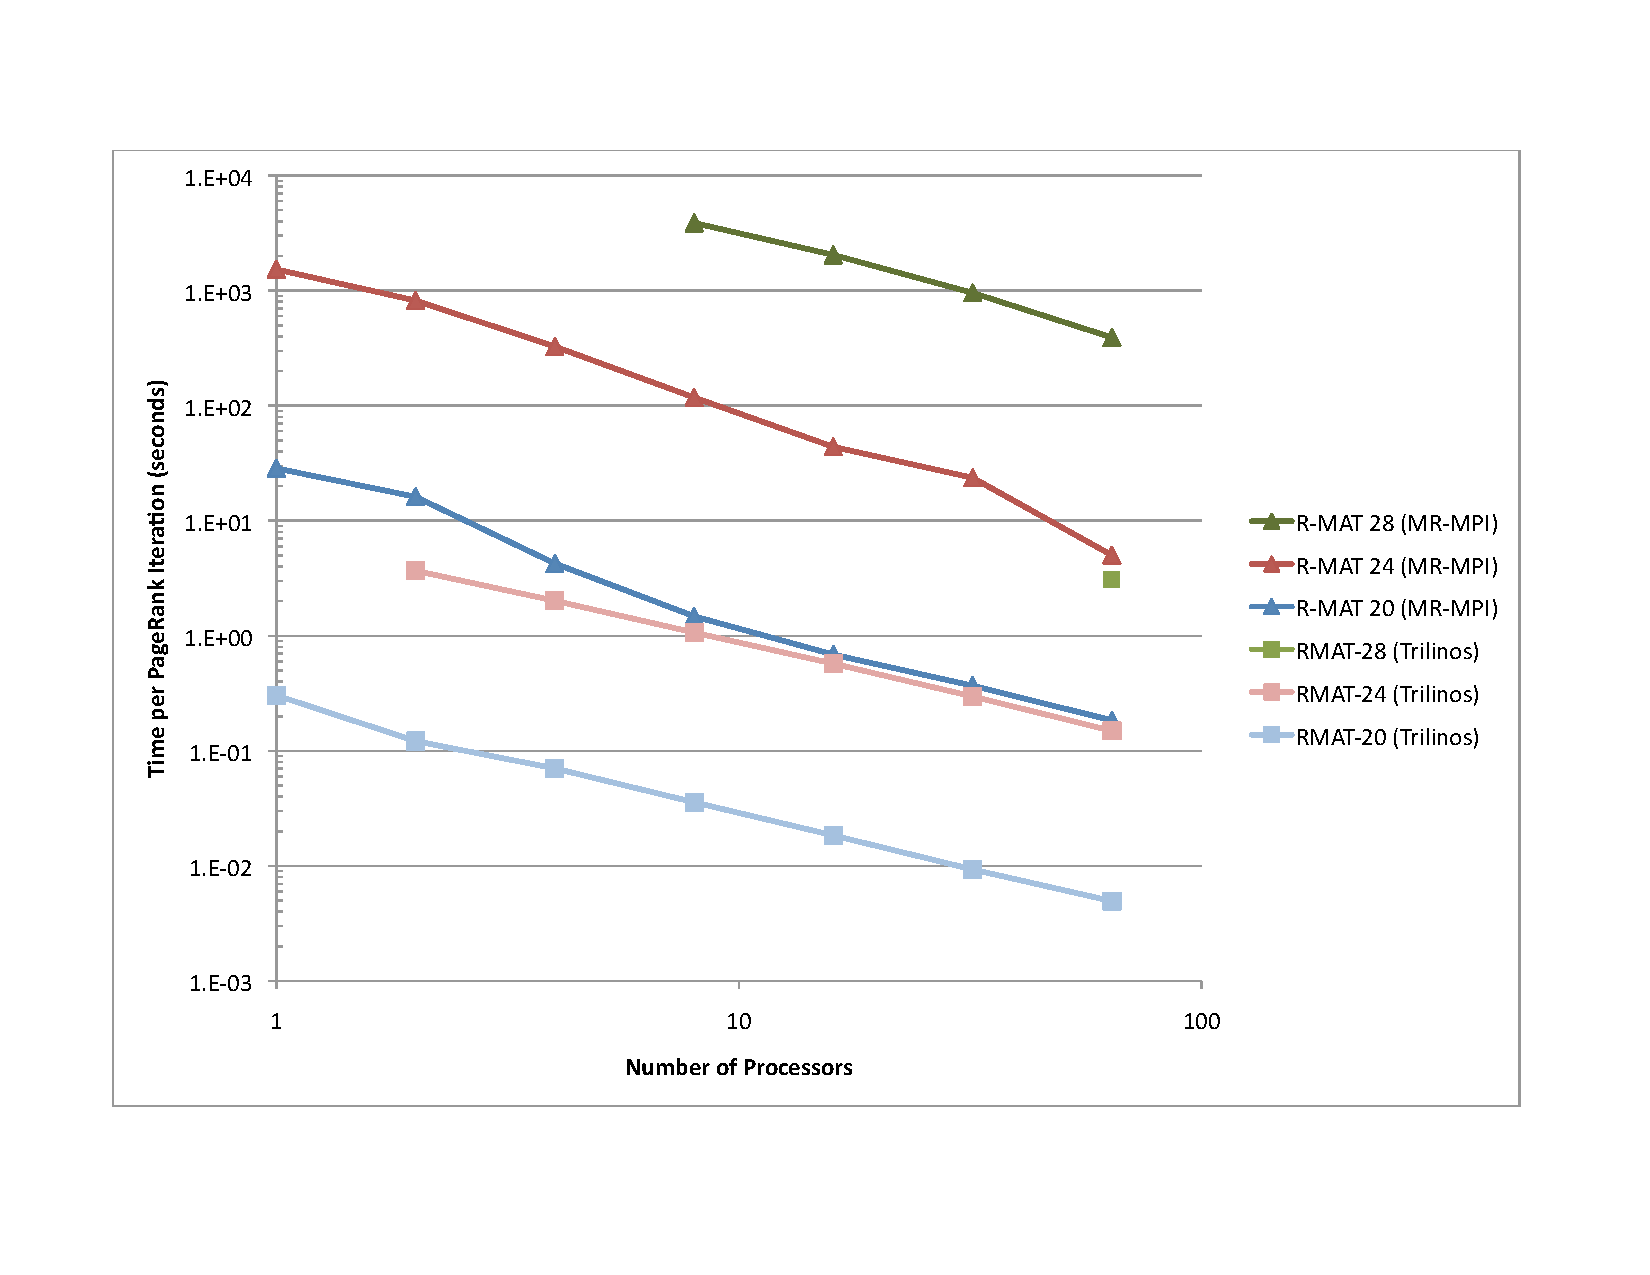
\includegraphics[width=\textwidth]{fig_pagerank.pdf}
\caption{Comparison of PageRank implementations using MapReduce,
Trilinos, and MTGL on R-MAT data sets.}
\label{f:prbig}
\end{figure}

